\section{Results: Explaining the Failure}
\label{sec:explaining}

\subsection{Near-Cancellation Structure}

The logit decomposition in S-059b measures each decoder cross-attention head's
contribution to the \texttt{I\_JUMP}$-$\texttt{I\_WALK} logit margin at the action-slot
divergence step, using a LayerNorm-corrected projection through T5's final decoder
RMSNorm ($n_\text{fail}=29$, $n_\text{success}=25$, SEED=42).
S-059 V0.1.0 pre-LayerNorm values (reconstruction fraction $\approx 32{,}193\times$)
are a methodological partial finding and are not used; all values in this section are
from S-059b.

The central finding is near-cancellation:
\begin{itemize}
  \item Mean reconstructed margin (cross-attention heads only): $-171.25$ logit units.
  \item Mean residual (FFN\,/\,embedding\,/\,self-attention correction): $+165.25$ logit units.
  \item Mean observed margin (\texttt{I\_JUMP}$-$\texttt{I\_WALK}): $-6.005$ logit units.
  \item Reconstruction fraction: $28.52\times$.
\end{itemize}
The cross-attention signal pushing toward \texttt{I\_WALK} is large and is opposed by
an almost equally large correction from the remaining residual stream components.
The model fails not by an unchallenged pro-walk drive, but by the small imbalance
remaining after near-cancellation of two large opposing terms.

Within the cross-attention decomposition, the four largest pro-walk contributors form
an L6 cluster: L6H2 ($\delta\mathrm{logit}=-51.21$, rank~1), L5H6 ($-40.56$, rank~2),
L6H6 ($-37.67$, rank~3), and L6H5 ($-29.61$, rank~4).
The S-051 target heads L5H5 ($-19.65$, rank~6) and L4H6 ($-10.41$, rank~8) also
contribute in the pro-walk direction but are smaller.
L6H7 ($+21.90$) is the largest pro-jump contributor.
The L3H0 diagnostic control head ($+2.98$ fail, $+3.21$ success, $\Delta=+0.23$) is
stable across groups, consistent with its non-causal role.
Fifty per cent of the negative cross-attention margin is accounted for by four heads
(through L6H5); 75\% by seven heads (through L4H6); 90\% by fourteen heads.

Figure~\ref{fig:near-cancellation} illustrates the near-cancellation structure.

\begin{figure}[t]
\centering
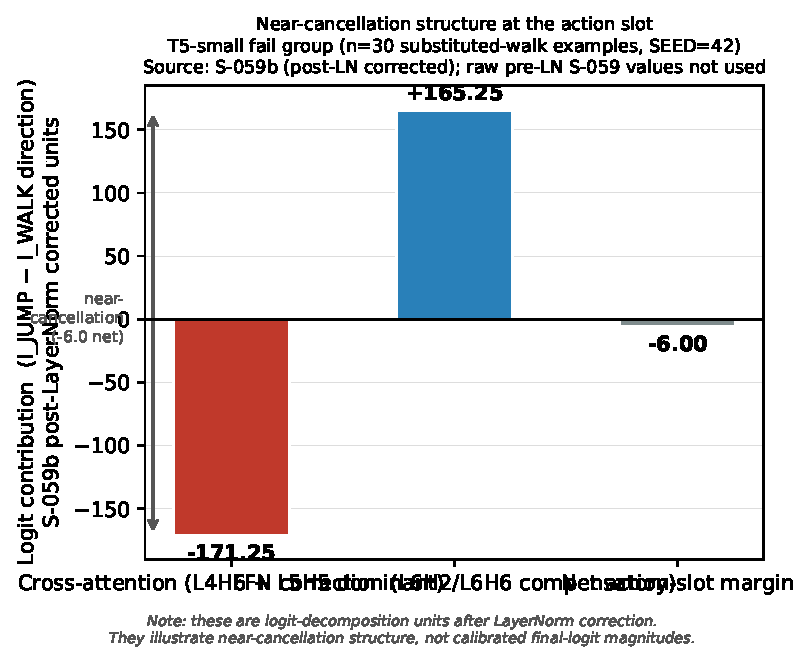
\includegraphics[width=0.68\linewidth]{figures/fig04_near_cancellation}
\caption{Near-cancellation structure at the action slot. T5-small fail group ($n=30$
substituted-walk examples, SEED=42). Values from S-059b post-LayerNorm corrected logit
decomposition (cited in \texttt{METHODS\_REPORT\_S061.md}).
These are logit-decomposition units after LayerNorm correction; they illustrate
near-cancellation structure, not calibrated final-logit magnitudes.
Pre-LayerNorm (S-059 V0.1.0) values are not used.}
\label{fig:near-cancellation}
\end{figure}

\subsection{Norm Asymmetry as Amplification}

The near-cancellation structure explains why a large pro-walk signal is only partially
offset.
A second mechanism explains why the small residual pro-walk margin produces extreme
output probabilities: $P(\texttt{I\_WALK})=0.914$, $P(\texttt{I\_JUMP})=0.002$ at the
divergence step in fail cases (S-050b).

The output embedding norms are asymmetric: $\|\texttt{I\_WALK}\|\approx 520$ versus
$\|\texttt{I\_JUMP}\|\approx 424$ (S-050b sealed measurement).
Raw logits are proportional to $\|e\|\cdot\cos(\mathbf{h},e)$; the larger norm of
\texttt{I\_WALK} amplifies even a modest positive cosine alignment into a dominant logit
under softmax.
S-051 Option~A (\S\ref{sec:locating}) confirms this norm lever is causally load-bearing:
equalizing all four action-token embedding norms to unit length collapses
$P(\texttt{I\_WALK})$ from $0.914$ to $0.323$, while the remaining tokens distribute
in the range $0.217$--$0.323$.
After normalization \texttt{I\_WALK} retains the highest probability, confirming that
a real directional bias toward \texttt{I\_WALK} persists in the hidden state independent
of the norm effect; the norm asymmetry is the amplification mechanism that converts a
small cosine lead into a dominant probability.

Together, near-cancellation (S-059b) and norm asymmetry (S-050b, S-051) describe two
stages: (1) a large pro-walk cross-attention signal is only partially offset by FFN
correction, leaving a small net pro-walk margin in the residual stream; (2) norm
asymmetry amplifies this small margin into the extreme action-token probabilities
observed at the divergence step.

\subsection{Compensatory Heads and Sign-Reversal Under Ablation}

Given the L6 cluster's dominance in the decomposition (\S\ref{sec:explaining}), S-060
tested whether L6H2 and L6H6 are causally upstream of the failure using within-example
neutralization: each head's V/O projection contribution was subtracted from the
residual stream within the fail example's own forward pass, and the change in logit
margin ($\Delta m$) was measured.

K1 fires: within-example neutralization does not isolate the L6 cluster as independent
causal agents.

Arm~A (L6H2) produced $\Delta\text{specificity}=-0.937$ ($n=29$): neutralizing a head
with $\delta\text{logit}=-51.21$ (pro-walk in the decomposition) \emph{worsened} the
logit margin, not improved it.
Arm~B (L6H6) showed the same sign ($\Delta\text{specificity}=-0.394$), and the joint
arm~C produced $\Delta\text{specificity}=-1.320$.
These heads are compensatory correctors, not error sources: their participation in the
near-cancellation structure is such that their removal tips the balance further toward
pro-walk, not toward pro-jump.

Two mechanisms are consistent with the sign-reversal.
First, \textbf{LN-rescaling disruption}: T5's final decoder RMSNorm rescales the full
residual stream before \texttt{lm\_head}.
L6H2 has the largest contribution norm of any head
($\|\mathrm{contrib}\|_{L6H2}\approx 1985$, $\|\mathrm{contrib}\|_{L6H6}\approx 1567$);
removing these contributions substantially alters the residual stream's RMS, changing
the LN scale factor for all remaining components non-linearly.
Second, \textbf{near-cancellation sensitivity}: when cross-attention ($-171$) and FFN
correction ($+165$) nearly cancel, removing one large cross-attention term can leave
the FFN correction uncompensated, driving the margin further negative.
Both mechanisms predict non-monotone, unpredictable effects from large-norm ablation
in this architecture.

The S-051 target heads show small positive specificity under the same instrument.
Arm~D (L4H6): $\Delta\text{specificity}=+0.121$ ($n=29$; $+0.132$ on $n=23$ excluding
six structurally fragile examples).
Arm~E (L5H5): $\Delta\text{specificity}=+0.180$ ($n=29$; $+0.229$ on $n=23$).
Both specificities grow modestly when fragile examples are excluded, and neither
disappears, but both remain far below K1 threshold ($0.50$).
Their moderate contribution norms ($\|\mathrm{contrib}\|_{L4H6}\approx 543$,
$\|\mathrm{contrib}\|_{L5H5}\approx 754$) produce proportionally smaller LN-rescaling
disruption, bringing the ablation response closer to linear prediction.
Arm~E specificity is interpretively weakened because the L5H4 control arm worsens the
margin ($\Delta m_\text{ctl}=-0.148$, $n=23$); the reported specificity therefore reflects
both L5H5's target-arm behavior and the negative control-arm baseline, not an isolated
L5H5 causal effect.

The S-060 lesson for instrument design: neither cross-example patching (S-058) nor
within-example neutralization of large-norm heads produces clean specificity signals
in a near-cancellation architecture with LN rescaling.
The small positive specificities of L4H6 and L5H5 motivated the targeted W$_V$
repair reported in \S\ref{sec:repair}.

\paragraph{Why the repair targets L4H6 and L5H5, not the L6 cluster.}
Decomposition rank identifies where the final logit margin is numerically concentrated;
it does not by itself identify clean intervention targets.
The L6 cluster (L6H2, L5H6, L6H6, L6H5) holds ranks 1--4 by $|\delta\text{logit}|$
(S-059b) but shows sign-reversed or negative specificity under within-example
neutralization (S-060: $\Delta\text{specificity}=-0.937$ for L6H2 and $-0.394$ for
L6H6), consistent with the LN-rescaling and near-cancellation confounds above rather
than a clean causal error source.
L4H6 and L5H5 were selected because they combined pro-walk value-direction evidence
(S-051) with small positive specificity under the same instrument
($+0.121$ and $+0.180$ at $n=29$) and a positive repair response under the rank-1
$W_V$ intervention (\S\ref{sec:repair}).
The repair targets are therefore not the largest decomposition terms; they are the
heads for which the current instrument gave a clean, directionally interpretable
intervention.

\subsection{G-Track Independent Confirmation (G-056, G-057)}

Two controlled toy geometry experiments, conducted independently from the S-track using
a 6-layer NumPy toy model (D=16; 8 geometric dims + 8 FIN dims; SEED=57), demonstrate
the same structural phenomena identified in the production system.
These results provide an analogy/convergence check, not a calibrated toy-to-production
prediction.

\paragraph{FIN-inversion mechanism (G-056).}
G-056 introduced a suppressive cross-attention head with value matrix
$W_V = I - \alpha \cdot P_\text{FIN}$ and swept $\alpha$ from 0 to~2.
At $\alpha=2.0$, the FIN component of the head output is inverted rather than suppressed.
The Born filter ablation change jumps to 42\% (versus 4\% at the neutral-head baseline
$\alpha=0$), driven by FIN-specialist layers downstream re-routing to amplify the
inverted signal.
This is value substitution at geometry scale: the head reads the correct encoder
position but its value projection maps the representation to the wrong output direction
--- the same structural property identified for L4H6 and L5H5 in S-051.

\paragraph{Near-cancellation divergence and sign-reversal (G-057).}
G-057 introduces an FFN correction parameter $\gamma$ that partially cancels the
cross-attention head's FIN contribution:
$\mathrm{FFN}(h)=h-\gamma\cdot P_\text{FIN}\cdot\mathrm{head\_output}$.
The reconstruction fraction ($\mathrm{head\_signal}/\mathrm{observed\_margin}$) is
$1.00\times$ at $\gamma=0$ by construction and diverges as $\gamma\to 1.0$:
$1.55\times$ at $\gamma=0.75$; $5.31\times$ at $\gamma=0.95$;
$\infty$ ($9{,}184\times$ measured) at $\gamma=1.0$.
This mirrors the production near-cancellation ($28.52\times$ in S-059b): in both
systems, a large primary signal is nearly canceled by an opposing correction, leaving
a small residual that determines the output.
At $\gamma=2.0$ (over-correction), G-057 reproduces the G-056 FIN-inversion at 51.3\%
ablation change, confirming that the inversion mechanism generalizes from value-matrix
to FFN-path perturbations.

G-057 also shows a directional analog to S-060's sign-reversal: ablating the corrective
FFN component worsens Born filter discrimination, while ablating the upstream head
improves it ($\gamma=0.90$: corrective $\Delta=-1.6\%$, upstream $\Delta=+0.8\%$;
$\gamma=0.95$: corrective $\Delta=-2.0\%$, upstream $\Delta=+0.5\%$).
The effect magnitude is below the pre-registered $\pm 5\%$ threshold because the
neutral global head's base signal is small.
This should be treated as directional consistency with the sign-reversal pattern,
not as a threshold-passing confirmation of H5.

Figure~\ref{fig:two-track} shows the two-track near-cancellation convergence.
Both systems --- T5-small's decoder (S-059b) and the NumPy toy (G-057) --- exhibit the
same structural property: a large cross-attention signal that is nearly canceled by an
opposing correction, leaving a small residual that determines the output.

\begin{figure}[t]
\centering
\includegraphics[width=\linewidth]{figures/fig07_two_track_near_cancellation}
\caption{Two-track near-cancellation convergence.
Panel~(A): Production measurement (S-059b, post-LayerNorm corrected) shows
near-cancellation in T5-small --- cross-attention $-171.25$ and FFN $+165.25$
cancel to leave net margin $-6.005$ (logit units after LN correction).
Panel~(B): Controlled toy geometry (G-057) independently demonstrates that
near-cancellation is a real regime as $\gamma \to 1.0$; reconstruction fraction
diverges from $1.00\times$ at $\gamma=0$ to $\infty$ ($9{,}184\times$ measured)
at $\gamma=1.0$.
This is an analogy/convergence claim, not a calibrated toy-to-production logit prediction.}
\label{fig:two-track}
\end{figure}

\subsection{What This Does Not Establish}

\begin{itemize}
  \item \textbf{Causal attribution to the L6 cluster.}
    L6H2, L5H6, L6H6, and L6H5 dominate the cross-attention decomposition (S-059b,
    ranks 1--4 by $|\delta\text{logit}|$) but show negative specificity under
    within-example neutralization (S-060).
    Their decomposition ranking is real; their causal status as independent
    error sources is not established by this instrument.

  \item \textbf{Causal attribution to L4H6 and L5H5.}
    The small positive specificities of Arm~D and Arm~E ($+0.12$ and $+0.18$ at
    $n=29$; $+0.13$ and $+0.23$ at $n=23$) are consistent with but do not prove
    that L4H6 and L5H5 are causally upstream.
    Both remain far below K1 threshold.
    The causal test at the weight level --- targeted W$_V$ modification ---
    is reported in \S\ref{sec:repair}.

  \item \textbf{Complete logit decomposition.}
    S-059b decomposes cross-attention heads only; FFN, self-attention, and embedding
    contributions are not individually decomposed.
    The reported $28.52\times$ value is the ratio between the cross-attention partial
    margin and the observed final margin, not a complete reconstruction of the final
    logit; the compensating FFN/embedding/self-attention correction is established in
    aggregate but not decomposed component-by-component.

  \item \textbf{Quantitative toy-to-production prediction.}
    The G-track convergence (G-056, G-057) is a structural analogy: both systems
    exhibit near-cancellation and value-direction substitution.
    No calibrated formula mapping toy Born filter ratios or logit gaps to production
    logit magnitudes is claimed.
    The two-track evidence strengthens the qualitative mechanistic account; it does
    not constitute a quantitative prediction.
\end{itemize}
